\chapter{Anexos}

\section{Lista de Abreviaturas}\zlabel{anexoabreviaciones}

\hspace{5mm} \textbf{API} \tab Application Programming Interface

\textbf{Cmake}\tab	Cross Platform Make (Make Multiplataforma)

\textbf{CUDA}\tab  Compute Unified Device Architecture

\textbf{DLL}\tab   Dynamic Link Library

\textbf{FPS}\tab  Frame per Second

\textbf{RAM}\tab  Random Access Memory

\textbf{GPU}\tab Graphic Processing Unit

\textbf{GUI}\tab  Graphical User Interface

\textbf{UI}\tab User Interface

\textbf{3D}\tab  3 Dimensiones

\textbf{CPU}\tab Central Processing Unit

\textbf{JPG-JPEG}\tab  Joint Photographic Experts Group 

\textbf{JSON}\tab  JavaScript Object Notation

\textbf{SDK}\tab  Software development kit

\textbf{txt}\tab  Plain Text


\newpage
\section{Glosario}\zlabel{anexoglosario}


\textbf{Algoritmo}: Un algoritmo se define como un conjunto de ordenes definidas y finitas con el objetivo de llegar a una solución a un problema, la realización de un computo, proceso de datos u otras actividades. El estudio de los algoritmos busca una constante mejora de la resolución de problemas empleando métodos distintos, con el fin de optimizar los recursos necesarios, así como una solución estandarizada y apropiada para un problema general.

\textbf{API}: Una API es una Interfaz de Programación de Aplicaciones, que es un conjunto de protocolos y definiciones empleada en el desarrollo e integración de Software que se emplea como una biblioteca.

\textbf{Animación}: La animación es el acto de producir imágenes en movimiento; técnica que significa que provee de movimiento a una grabación o una serie de dibujos (Oxford English Dictionary). 

\textbf{Código}: El código en el contexto, se define como el conjunto de símbolos y signos que se transmiten de un emisor a un receptor, cuya intención es privar del conocimiento de su contenido a terceros. Un código tiene un conjunto de reglas o normas que se emplean para dificultar la lectura del mensaje, siendo un ejemplo la traducción de un mensaje en español a ingles, el mensaje puede ser solo entendido por quien conozca el idioma ingles.

\textbf{Cmake}: Es una herramienta multiplataforma de automatización o generación de código.

\textbf{CPU}: La unidad central de procesamiento, es un Hardware requerido por una computadora o dispositivo Von Newmann, se encarga interpretar las ordenes de un Software o programa mediante operaciones aritméticas, lógicas y otros.

\textbf{CUDA}: Cuda se emplea para referenciar una plataforma de computación en paralelo, con compilador y herramientas de desarrollo creado por la compañia nVidia.

\textbf{Dataset}: Un dataset es una tabla dentro de una base de datos, en la cual se representa una variable particular en la primera columna, y cada fila es un componente del conjunto de datos.

\textbf{DLL} Una biblioteca de enlace dinámico es un archivo con código ejecutable para poder utilizar programas por el sistema operativo.

\textbf{Decodificador}: El decodificador es una herramienta que permite descifrar un mensaje codificado. Se refiere a la actividad inversa de la codificación, implica la recepción de un código y de acuerdo al conjunto de normas establecidas para su traducción, se lo interpreta y se obtiene el mensaje inicial que se deseaba recibir.

\textbf{Frame}: Las grabaciones o serie de dibujos están compuestas por cuadros o Frames en ingles, que son una imagen individual de la secuencia de imágenes que componen la animación para dar la sensación de movimiento. La mayoría de las animaciones emplean de 24 a 30 Frames per second (FPS). 

\textbf{Framework}: El Framework es toda estructura conceptual y tecnológica de soporte definido, con artefactos o módulos de Software que sirven para la el desarrollo y organización de Software.

\textbf{Hardware}: El Hardware se entiende como el componente físico de una computadora o dispositivos de Von Neumann. Esta compuesto por el procesador, la tarjeta madre, RAM, disco duro, monitor, dispositivos de entrada y salida, los cuales normalmente se mencionan como componentes y a los dispositivos externos como periféricos\cite{hardwaredef}.

\textbf{GPU}: La unidad de procesamiento gráfico es un procesador suplementario al  central, aligera la carga para trabajar con gráficos u operaciones de tipo flotante, normalmente usado en aplicaciones 3D interactivas. 

\textbf{GUI}: Una interfaz gráfica de usuario es una interfaz diseñada con imágenes y gráficos para la representación de la información y controles disponibles en la interfaz del usuario.

\textbf{UI}: La interfaz puede ser usada tanto en un contexto de Hardware o de usuario, siendo la segunda la definición relevante.
Una interfaz de usuario tiene la función de otorgar al usuario el control de una aplicación de Software o un dispositivo de Hardware. Uno de los objetivos de la UI es ser amigable con el usuario, permitiendo interactuar con la aplicación de manera intuitiva y natural. Ejemplos de UI pueden ser la pantalla de inicio de una pagina web y de Hardware un control remoto de televisión.

\textbf{JPG}: Es un formato estándar de codificación y compresión de imágenes y archivos estáticas. JPG es una abreviación de Joint Photographic Experts Group (JPEG), comité que creo dicho formato.

\textbf{JSON}: El JavaScript Object Notation es un formato ligero e independiente de lenguajes para la transmisión de datos, es de simple lectura y fácil para el procesamiento de la máquina.

\textbf{Software}:El software esta construido para ejecutar dispositivos von Neumann multiproposito. Un software contienen secuencias de declaraciones de programas abstractos que describen las tareas que deben ser realizadas por una maquina. 

\textbf{Modelo de Von Neumann}: Es una arquitectura de computadoras, su objetivo es explicar como funciona una computadora y la interacción entre sus distintos componentes (CPU, RAM y otros).

\textbf{Interprete}:El interprete en el contexto informático es un programa traductor que permite ejecutar otros programas a lenguaje máquina, a diferencia de los compiladores, estos solo ejecutan la sección que requieren emplear.

\textbf{Pixel}: El pixel es la unidad mínima homogénea en color que en su conjunto da forma a una imagen digital.

\textbf{Plug-in}: Un plug-in o complemento es un Software o Aplicación con un grupo de características y funciones especificas para interactuar por medio de una API.

\textbf{RAM}: La memoria de acceso aleatoria se emplea para guardar los datos de trabajo temporal de la computadora y demás para el sistema operativo, el Software y los programas que se ejecutan, la RAM carga con todas las instrucciones que ejecuta el CPU para trabajar con los distintos programas.

\textbf{Shell}: Shell es un interprete de comandos para acceder y emplear los servicios del sistema operativo, son necesarios para ejecutar los programas de una computadora.

\textbf{Script}: El script es una secuencia de comandos, estos son ejecutados primero por un interprete que lee el codigo fuente o una consola interactiva para que el usuario trabaje. Se los utiliza para automatizar tareas repetitivas, interactuar con el sistema operativo y otros.

\textbf{SDK}: El kit de desarrollo de Software es un conjunto de herramientas para el desarrollo de Software, permite la creación de una aplicación para sistemas concretos, es una API creada para poder usar ciertos lenguajes de programación y en algunos casos, comunicarse con ciertos sistemas embebidos, en algunos casos, son capaces de detectar errores y aportar utilidades extra.

\textbf{txt}: El txt es el formato de los documentos de texto plano.





\clearpage
\begin{landscape}
	\section{Anexo: Control de Sprint}\zlabel{anexosprint}
	\begin{figure}[b!]
		\centering
		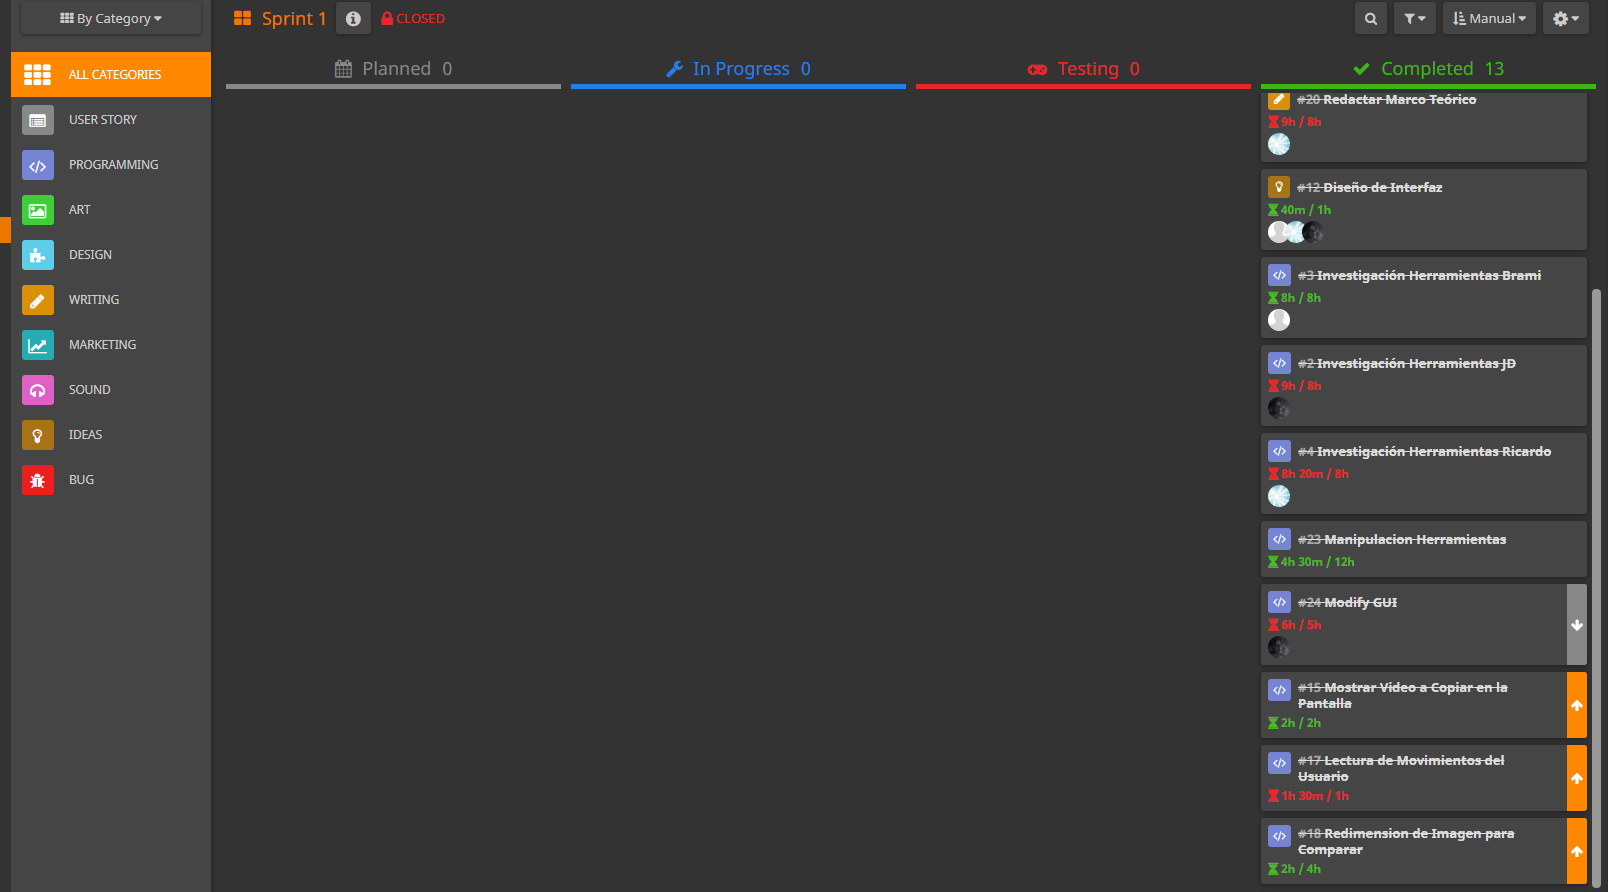
\includegraphics[width=20cm,height=12cm,]{./Images/sprintexample2.png}
		\caption{Sprint 1 concluida}
		\footnotesize Fuente: Elaboración Propia empleando la herramienta HacknPlan.
		\label{sprintexample2}
	\end{figure}
	
	\clearpage
	\begin{figure}[t!]
		\centering
		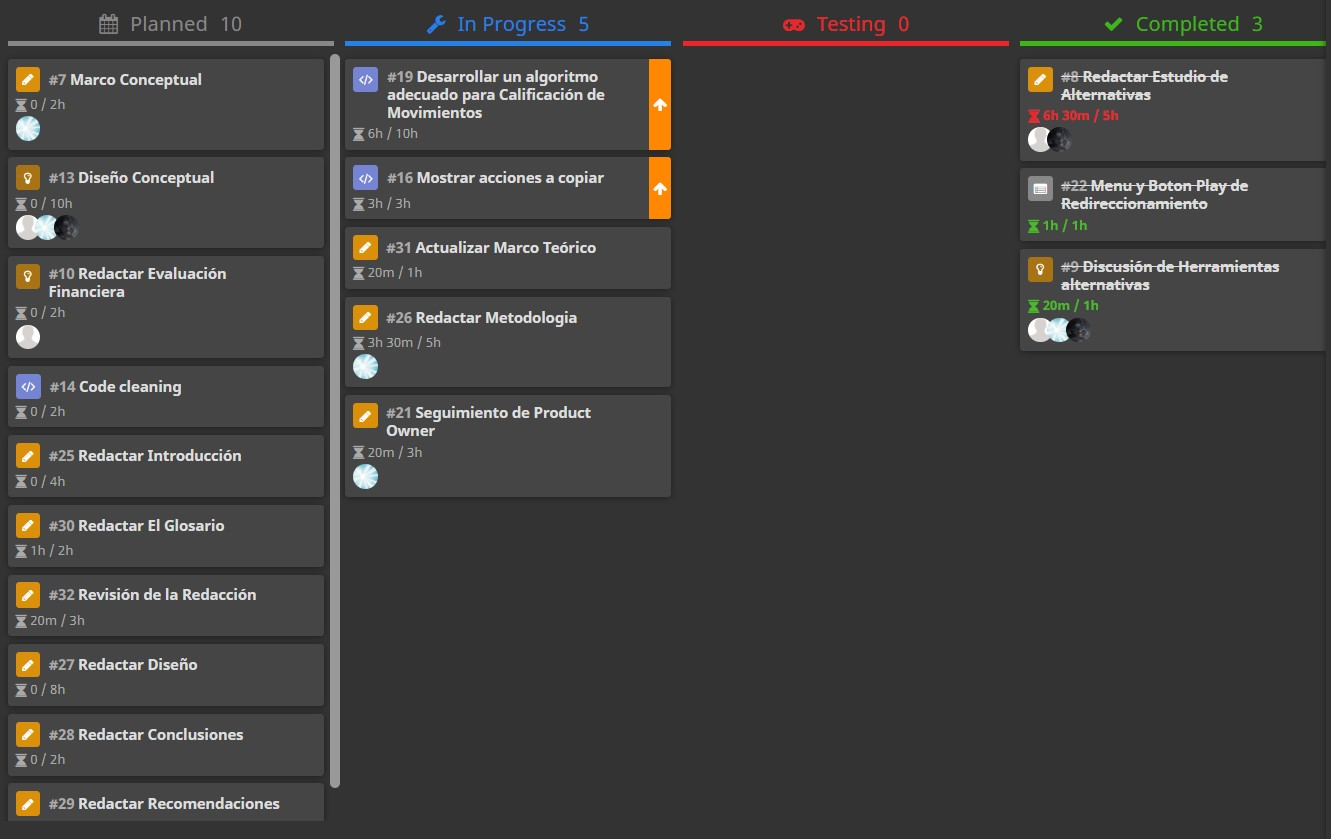
\includegraphics[width=23cm,height=15cm,]{./Images/hacknplanexample.jpg}
		\caption{Sprint Backlog del día 5 de Noviembre}
		\footnotesize Fuente: Elaboración Propia empleando la herramienta HacknPlan.
		\label{sprintexample}
	\end{figure}
	
\end{landscape}

\clearpage
\begin{figure}[t!]
	\centering
	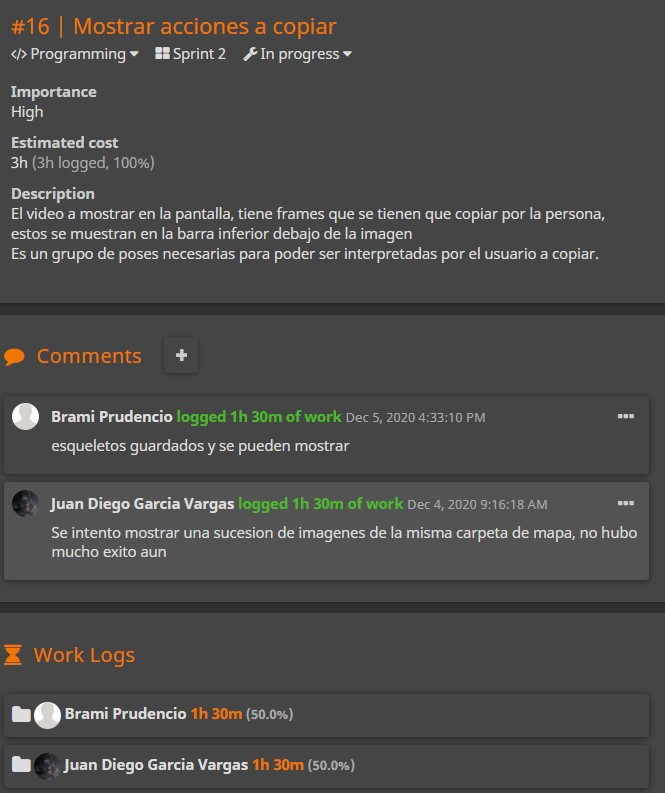
\includegraphics[width=15cm,height=20cm,]{./Images/tareaexample.jpg}
	\caption{Tarea de la Sprint 2, Mostrar Acciones a Copiar}
	\footnotesize Fuente: Elaboración Propia empleando la herramienta HacknPlan.
	\label{sprinttarea}
\end{figure}

\clearpage
\section{Anexo: Product Backlog} \zlabel{anexoproduct}
En la tabla \ref{productbacklog} del Product Backlog, se observan los campos:
\begin{itemize}
	\item ID como identificador de la tarea, debe ser único.
	\item Tarea, que indica el título dado en Sprint Backlog para facilitar su comprensión.
	\item Estado(Sprint), si ha de estar Planificada, En Proceso o Hecho (Sprint en que se realizo) o si fue Descartado.
	\item Valor, el valor designado a cada actividad realizada, en total se asignan 1000 puntos a su finalización
	\item Estimado Inicial, la valoración de las tareas que se mide en horas requeridas.
	\item Factor Ajuste, determina el fallo que se debe aumentar al tiempo original, se le suma al Valor Estimado en función $Valor Estimado = Valor Estimado + Valor Estimado * Factor de Ajuste$
	\item Ajustado, es la valoración de las tareas posteriormente al ser más realistas sobre el tiempo requerido para resolverlo.
	\item Sprint, que señala el número de Sprint en que fue realizada
	\item Prioridad, al ser una metodología ágil, se reconoce que las tareas pueden ser más relevantes unas que otras, en este caso, Baja, Normal y Alta.
	
\end{itemize}
La Tarea es el nombre dado a las tareas distribuidas al SCRUM Team, formuladas a partir de los requerimientos del cliente.
El valor de las tareas se distribuirá de un valor total de 1000 puntos, se determinara una cuarta parte a la redacción del informe, una cuarta parte a la investigación dedicada requerido para poder hacer posible el proyecto y el resto lo determinará el rol de Product Owner.
El Estimado Inicial es definido con la Estimación de Poker previamente mencionada.
Redactar en la tabla \ref{productbacklog} engloba la redacción del informe y el tiempo estimado de cada tarea de redacción, el Redactar hace referencia a los títulos de cada parte del informe.
En Redactar Parte 1, están los títulos de Objetivos, Estudio de Diagnóstico, Marco Teórico, Estudio de Alternativas, Plan de Actividades
En Redactar Parte 2, están los títulos de Metodología, Diseño, Conclusiones, Recomendaciones, dentro de la metodología se lleva a cabo la tarea de Seguimiento de Product Owner.
En Redactar Parte 3, están los títulos de Introducción, Anexos, Glosario, Revisión de ortografía y Resumen.
\restoregeometry
\newgeometry{left=0.5cm,bottom=.25cm}
\begin{landscape}
	\begin{table}[t]
		\begin{center}
			\begin{tabular}{| c | c | c | c | c | c | c | c | c |}
				\hline
				\multicolumn{9}{ |c| }{Product Backlog} \\ \hline
				ID & Tarea & Estado(Sprint) & Valor & Estimado Inicial (h)& Factor Ajuste & Ajustado(h) & Sprint & Prioridad \\ \hline
				T-0 & Redactar Parte 1 & Hecho(1) & 50 & 18 & 1.5 & 40 & 1 & Normal \\ \hline
				T-1 & Redactar Parte 2 & En proceso(2) & 100 & 20 &  &  & 2 & Normal \\ \hline
				T-1 & Redactar Parte 3 & En proceso(3) & 100 & 9 &  &  & 3 & Normal \\ \hline
				T-2 & Investigación de Herramientas & Hecho(1) & 250 & 24 & 3.0 & 96 &  1 & Normal \\ \hline
				T-3 & Manipulación de Herramientas & Hecho(1) &  & 12 & 1.0 & 24 & 1 & Normal \\ \hline
				T-4 & Modificación de GUI & Hecho(1) &  &  & &  & 1 & Baja \\ \hline
				T-5 & Mostrar Vídeo a Copiar en la Pantalla & Hecho(1) &  &  & &  & 1 & Alta \\ \hline
				T-6 & Lectura de Movimientos del Usuario & Hecho(1) &  &  & &  & 1 & Alta \\ \hline
				T-7 & Redimension de Imagen para Comparar & Hecho(1) &  &  & &  & 1 & Alta \\ \hline
				T-8 & Menú y Boton Play de Redireccionamiento & Hecho() &  &  & &  &  & Baja \\ \hline
				T-9 & Calificación de Movimientos & Hecho(2) &  & 10 &  &  & 2 & Alta \\ \hline
				T-10 & Mostrar acciones a imitar & Hecho(2) &  & 3 & &  &  & Alta \\ \hline
				T-11 &  & &  &  & &  &  & Normal \\ \hline
				& Entrega final & & 1000 &  &  &  &  &  \\ \hline
			\end{tabular}
			\caption{Product Backlog}
			\label{productbacklog}
			\footnotesize Fuente: Elaboración propia
		\end{center}
	\end{table}
\end{landscape}
\restoregeometry


\clearpage
\section{Anexo: Gráfico Burn-Up Burn-Down}\zlabel{anexoburn}
\begin{figure}[b!]
	\centering
	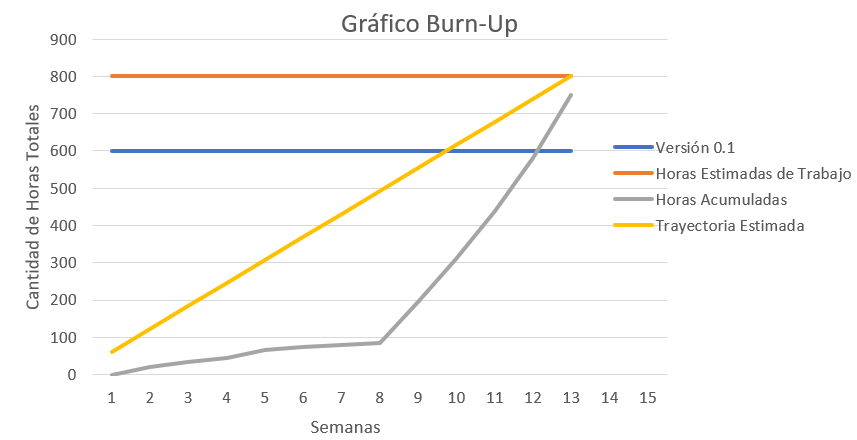
\includegraphics[width=14cm,height=8cm,]{./Images/graficoburnup.png}
	\caption{Gráfico Burn-Up}
	\footnotesize Fuente: Elaboración Propia
	\label{burnup}
\end{figure}
\begin{figure}[b!]
	\centering
	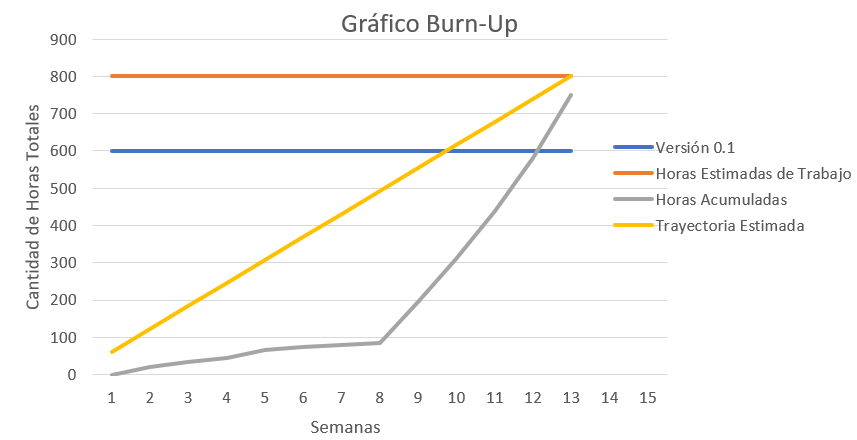
\includegraphics[width=14cm,height=8cm,]{./Images/graficoburnup.png}
	\caption{Gráfico Burn-Down}
	\footnotesize Fuente: Elaboración Propia
	\label{burndown}
\end{figure}


\newpage
\section{Anexo: Proceso de Instalación de OpenPose y Unity para el Desarrollo del Proyecto}\zlabel{anexoinstalacion}

Inicialmente se deben instalar la SDK de Visual Studio 2019 , de la pagina oficial  \href{https://visualstudio.microsoft.com/es/thank-you-downloading-visual-studio/?sku=Community&rel=16}{visualstudio.microsoft.com}, se ejecuta el archivo, se selecciona el paquete de idioma deseado y se lo descarga.

Posteriormente, se debe seleccionar la versión deseada, en este caso se trabajo con "Visual Studio Community 2019", se deben habilitar las opciones prrincipales de "Desarrollo de .NET", "Desarrollo para el escritorio con C++", "Desarrollo de juego con Unity", para realizar este proyecto. Se tiene que habilitar todas las opciones relacionadas con C++ y las Build Tools VS 2015-2017 en "Desarrollo para el escritorio con C++" como se observa en la figura \ref{vsinstall} de \ztitleref{anexoinstalacion}, ya que OpenPose las utiliza, finalmente se lo debe instalar en el lugar deseado y ejecutar.


\begin{figure}[t!]
	\centering
	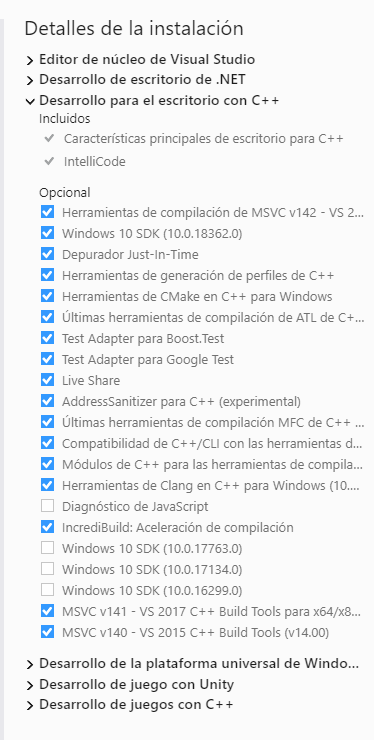
\includegraphics[width=8cm,height=16cm,]{./Images/eleccionesvsinstall.png}
	\caption{Elección Personal del Estudiante para Configurar Visual Studio 2019}
	\footnotesize Fuente: Instalador de Visual Studio.
	\label{vsinstall}
\end{figure}

La instalación de Unity inicia vistiando su pagina oficial de descargas  \href{https://unity3d.com/es/get-unity/download}{unity3d.com/es/get-unity/download}, se selecciona la opción de Descarga Unity Hub, se selecciono la opción "Personal" y de "Usuario recurrente", finalmente se aceptan los términos y condiciones, para descargar el instalador, se lo ejecutara y configurara como se desee, se debe ejecutar el programa instalado "Unity Hub".  

En la página oficial de versiones existentes \href{https://unity3d.com/get-unity/download/archive}{unity3d.com/get-unity/download/archive}, se seleccionara la versión Unity 2019.4.14 y se selecciona la opción "Unity Hub", finalmente se acepta instalar la versión correcta, si se siguieron correctamente los pasos, se tendrá la instalación de la figura \ref{installunity} de \ztitleref{anexoinstalacion} al finalizar.

La herramienta de Body Tracking OpenPose tiene requisitos elevados para su instalación y desarrollo, si bien instalar el programa para modificar el código fuente original puede realizarse siguiendo las instrucciones de  \href{https://github.com/CMU-Perceptual-Computing-Lab/openpose/blob/master/doc/installation/README.md}{openpose/doc/installation/README.md} guardado en el repositorio principal de GitHub (CMU-Perceptual-Computing-Lab/openpose). Sin embargo, se empleara su plug-in de Unity almacenado en el repositorio  \href{https://github.com/CMU-Perceptual-Computing-Lab/openpose\_unity\_plugin}{CMU-Perceptual-Computing-Lab/openpose\_unity\_plugin} de GitHub.
Se deben realizar x pasos para instalarlo, básicamente seguir las instrucciones de su documentación de instalación. Primero descargar el repositorio de GitHub, ejecutar el archivo "getPlugins.bat", "getModels.bat" y "testBinary.bat" dentro de la carpeta, para descargar los modelos, los archivos binarios de OpenPose y una Demo que se nombrará como \textbf{OpenPoseDemo} con la cual realizar pruebas. 
Finalmente se abre la escena "Demo.Unity" localizada en ./OpenPosePlugin/Assets/OpenPose/Examples/Scenes/ en Unity y ejecutarla, si se realizo correctamente, se le pedirán aceptar dos problemas debido al versionamiento y será dirigido a la siguiente pantalla de Unity de las figuras \ref{unitydemo} y \ref{unitydemoexample}.
\begin{figure}[t!]
	\centering
	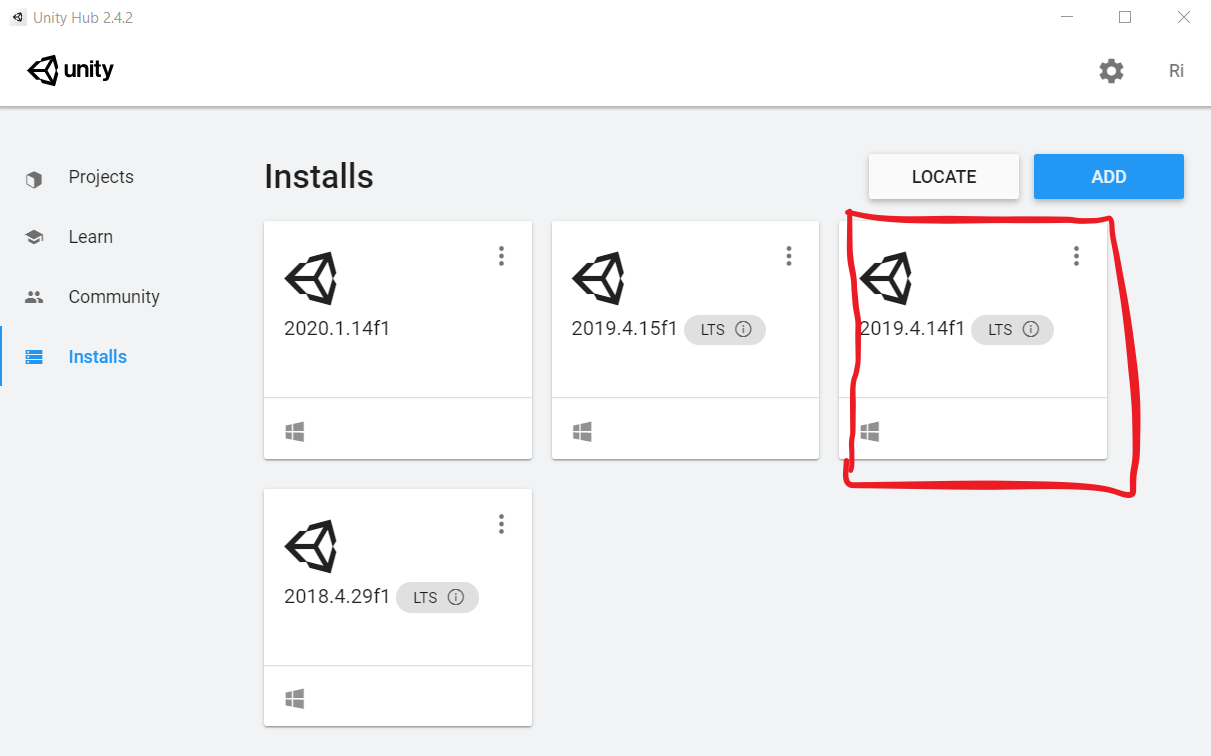
\includegraphics[width=12cm,height=8cm,]{./Images/installunity.png}
	\caption{Version Deseada de Unity Encerrada en Rojo}
	\footnotesize Fuente: Captura de Pantalla de Installs - Unity Hub.
	\label{installunity}
\end{figure}
\begin{figure}[t!]
	\centering
	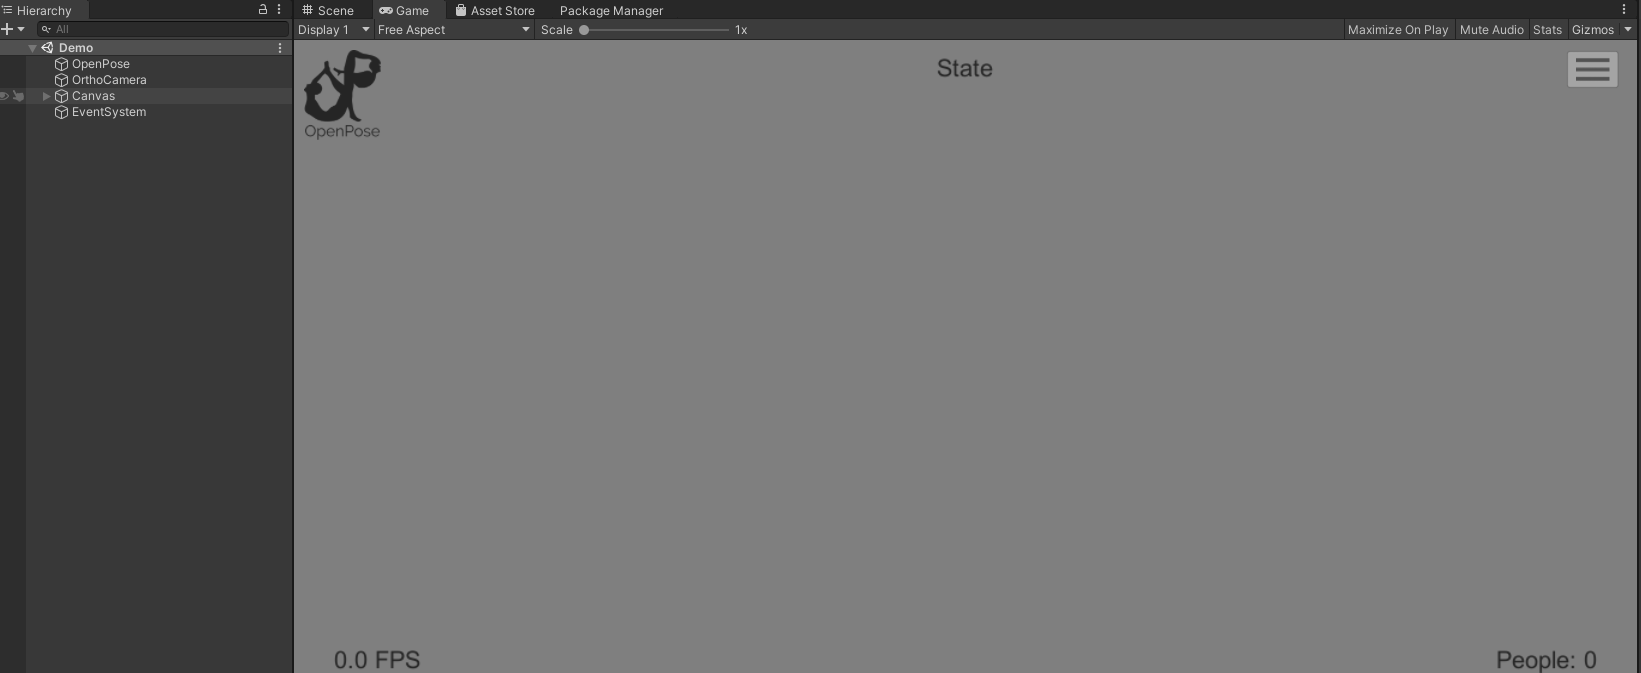
\includegraphics[width=15cm,height=7cm,]{./Images/unitydemo.png}
	\caption{Captura de Pantalla de la Configuración Inicial de OpenPose Plug-in}
	\footnotesize Fuente: Elaboración Propia Basado en \cite{8765346}
	\label{unitydemo}
\end{figure}
\clearpage
\null

\begin{figure}[t!]
	\centering
	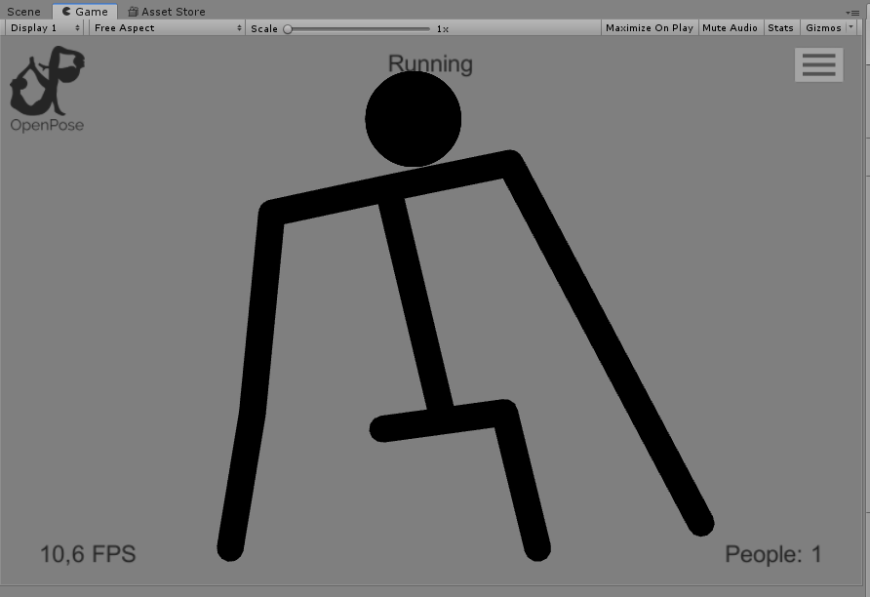
\includegraphics[width=14cm,height=8cm,]{./Images/ejemploopenunity.png}
	\caption{Prueba de Ejecución de Demo de OpenPose}
	\footnotesize Fuente: Elaboración Propia Basado en \cite{8765346}
	\label{unitydemoexample}
\end{figure}


\begin{landscape}
	\clearpage
	\section{Anexo: Archivos Generados}\zlabel{anexogenerados}
	\begin{figure}[b!]
		\centering
			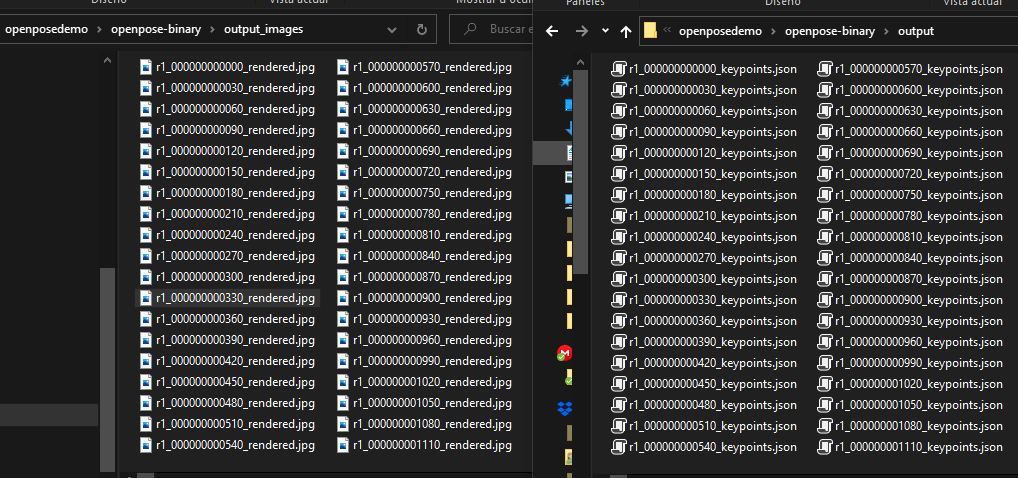
\includegraphics[width=22cm,height=12cm,]{./Images/JSONandJPGexample.png}
		\caption{Archivos Generados por la Conversión usando el Script con OpenPoseDemo}
		\footnotesize Fuente: Elaboración Propia Basado en \cite{8765346}
		\label{videotojsonpjg}
	\end{figure}
\clearpage
\section{Anexo: Mensajes de Error}\zlabel{anexoerrores}
	\begin{figure}[h!]
		\centering
		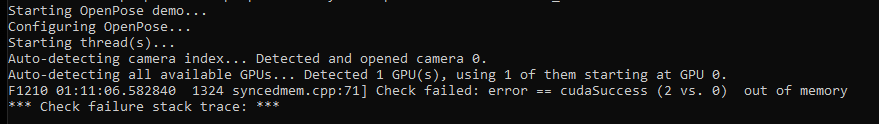
\includegraphics[width=22cm,height=5cm,]{./Images/erroroutofmemory.png}
		\caption{Archivos Generados por la Conversión usando el Script con OpenPoseDemo}
		\footnotesize Fuente: Elaboración Propia Basado en \cite{8765346}
		\label{erroroutofmemory}
	\end{figure}
\end{landscape}

\clearpage
\section{Anexo: Cálculos de Comparación de Poses}\zlabel{anexocomparacion}

\subsection{Ejemplo de Cálculo de Normalización Basada en el Centro de la Cadera}\zlabel{anexocadera}

Se tiene un vídeo grabado por un estudiante a medida que la lectura de Frames es dada, se guardaron 8 Frames selectos de manera arbitraria para la comparación de poses ilustrados en las figuras \ref{checker1} y \ref{checker2}, los cuales tienen los puntos clave en las tablas \ref{checkeroriginalpart1} \ref{checkeroriginalpart2} \ref{checkeroriginalpart3} \ref{checkeroriginalpart4}.

Los cálculos del porcentaje de semejanza entre el T Original con cada Frame selecto esta en las tablas \ref{checkerporcentage1} \ref{checkerporcentage2} \ref{checkerporcentage3} \ref{checkerporcentage4}, los cuales se emplearan para la ecuación \ref{equation3} dando los resultados de la tabla \ref{resultadoschecker}, donde T Original tiene un 100 \% de similitud y la diferencia independientemente de si es mayor o menor es la diferencia, como se puede ver solo hay un aproximado de 108 \% en el Frame 147 Dab, lo cual indica solo un aproximado de 8 \% de diferencia para poses tan distintas, convirtiendo este método de cálculo en uno muy inefectivo para poses distintas, pero bueno para poses similares en distintos lugares.

\begin{figure}[ht]
	\centering
	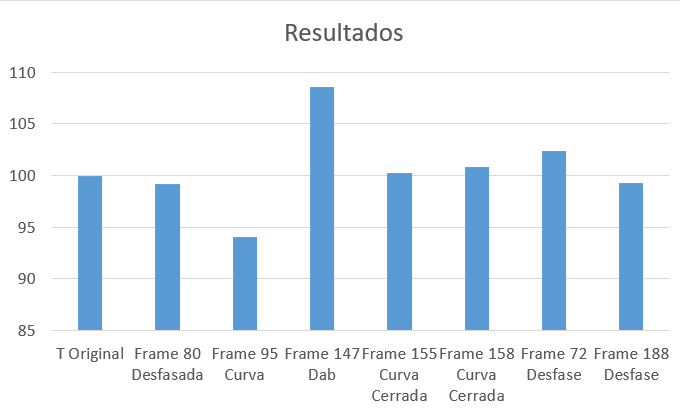
\includegraphics[width=12cm,height=7cm]{./Images/resultadoschecker.png}
	\caption{Tabla de Diferencias entre Poses}
	\footnotesize Fuente: Elaboración Propia
	\label{resultadoschecker}
\end{figure}

\begin{figure}[ht]
	\centering
	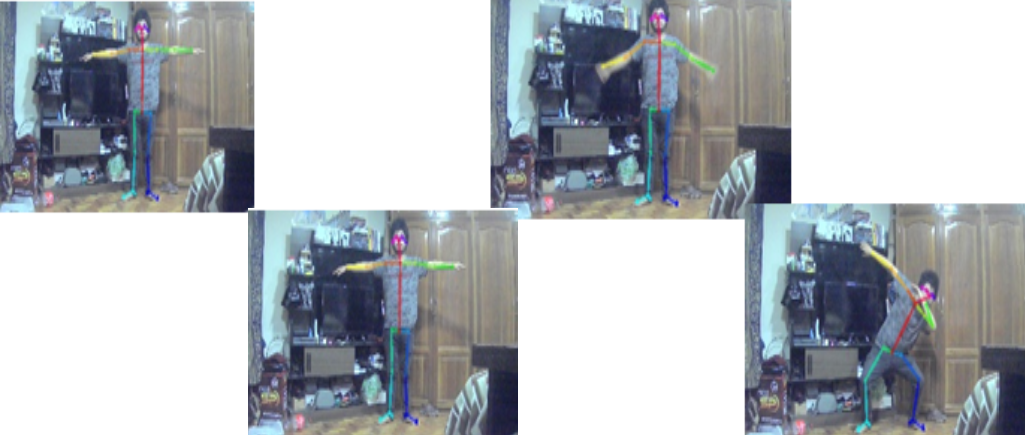
\includegraphics[width=16cm,height=10cm,]{./Images/checkerpart1.png}
	\caption{Poses: T Original - Frame 80 - Frame 95 Curva - Frame 147 Dab}
	\footnotesize Fuente: Elaboración Propia
	\label{checker1}
\end{figure}

\begin{figure}[ht]
	\centering
	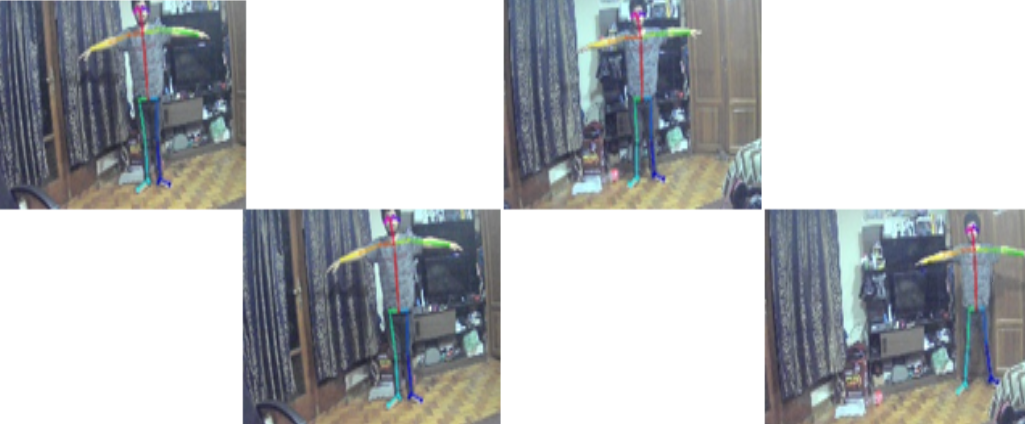
\includegraphics[width=16cm,height=10cm]{./Images/checkerpart2.png}
	\caption{Poses: Frame 155 Curva Cerrada - Frame 158 Curva Cerrada - Frame 72 Desfase - Frame 188 Desfase}
	\footnotesize Fuente: Elaboración Propia
	\label{checker2}
\end{figure}

\clearpage
% Table generated by Excel2LaTeX from sheet 'test'
\begin{table}[htbp]
	\centering
	\begin{tabular}{|l|c|c|}
		\hline
		Coordenadas & T Original & Frame 80\\ \hline 
		(x-0 ; y-0) & (713,549 ; 94,5737) & (713,713 ; 82,6751) \\
		(x-1 ; y-1) & (717,589 ; 165,122) & (719,531 ; 155,226) \\
		(x-2 ; y-2) & (650,932 ; 165,16) & (651,021 ; 155,255) \\
		(x-3 ; y-3) & (560,829 ; 178,768) & (560,901 ; 166,911) \\
		(x-4 ; y-4) & (474,593 ; 180,826) & (476,567 ; 168,975) \\
		(x-5 ; y-5) & (789,967 ; 165,069) & (790,029 ; 155,17) \\
		(x-6 ; y-6) & (878,214 ; 165,17) & (880,181 ; 166,925) \\
		(x-7 ; y-7) & (964,378 ; 167,014) & (964,378 ; 167,014) \\
		(x-8 ; y-8) & (713,711 ; 378,593) & (715,662 ; 370,634) \\
		(x-9 ; y-9) & (676,377 ; 374,707) & (678,356 ; 366,775) \\
		(x-10 ; y-10) & (678,369 ; 511,872) & (680,362 ; 498,068) \\
		(x-11 ; y-11) & (668,569 ; 647,009) & (668,713 ; 631,277) \\
		(x-12 ; y-12) & (758,596 ; 380,551) & (758,761 ; 370,707) \\
		(x-13 ; y-13) & (743,08 ; 515,78) & (745,016 ; 507,78) \\
		(x-14 ; y-14) & (746,985 ; 646,956) & (748,931 ; 635,116) \\
		(x-15 ; y-15) & (698,038 ; 84,7163) & (699,969 ; 72,8773) \\
		(x-16 ; y-16) & (727,333 ; 84,786) & (729,288 ; 72,9199) \\
		(x-17 ; y-17) & (682,286 ; 96,5211) & (684,223 ; 88,577) \\
		(x-18 ; y-18) & (745,001 ; 100,351) & (746,995 ; 90,481) \\
		(x-19 ; y-19) & (792,074 ; 674,425) & (795,937 ; 662,601) \\
		(x-20 ; y-20) & (793,917 ; 666,537) & (795,929 ; 654,715) \\
		(x-21 ; y-21) & (739,089 ; 654,823) & (741,057 ; 642,991) \\
		(x-22 ; y-22) & (621,554 ; 668,531) & (627,446 ; 654,804) \\
		(x-23 ; y-23) & (621,554 ; 664,564) & (625,515 ; 650,806) \\
		(x-24 ; y-24) & (680,334 ; 656,804) & (682,303 ; 641,062) \\ \hline 
	\end{tabular}%
	\caption{Puntos Clave T Original -  Frame 80}
	\footnotesize Fuente: Elaboración Propia
	\label{checkeroriginalpart1}
\end{table}%

% Table generated by Excel2LaTeX from sheet 'test'
\begin{table}[htbp]
	\centering
	\begin{tabular}{|l|c|c|}
		\hline
		Coordenadas &Frame 95 Curva &Frame 147 Dab	\\ \hline 
		(x-0 ; y-0) & (729,331 ; 4,366) & (978,154 ; 143,52) \\
		(x-1 ; y-1) & (735,144 ; 78,871) & (917,42 ; 163,131) \\
		(x-2 ; y-2) & (670,464 ; 76,91) & (884,023 ; 125,923) \\
		(x-3 ; y-3) & (586,208 ; 127,81) & (809,644 ; 59,34) \\
		(x-4 ; y-4) & (494,206 ; 153,34) & (727,409 ; 14,161) \\
		(x-5 ; y-5) & (797,855 ; 84,667) & (956,564 ; 200,389) \\
		(x-6 ; y-6) & (876,223 ; 131,712) & (993,837 ; 231,704) \\
		(x-7 ; y-7) & (964,378 ; 167,014) & (964,378 ; 167,014) \\
		(x-8 ; y-8) & (731,243 ; 290,389) & (813,554 ; 309,996) \\
		(x-9 ; y-9) & (694,018 ; 288,428) & (774,314 ; 296,356) \\
		(x-10 ; y-10) & (695,949 ; 421,716) & (694,038 ; 394,327) \\
		(x-11 ; y-11) & (684,197 ; 556,86) & (699,909 ; 517,78) \\
		(x-12 ; y-12) & (774,278 ; 290,431) & (854,677 ; 317,93) \\
		(x-13 ; y-13) & (758,684 ; 429,497) & (933,02 ; 390,453) \\
		(x-14 ; y-14) & (762,595 ; 556,875) & (905,618 ; 513,83) \\
		(x-15 ; y-15) & (715,549 ; -5,509) & (968,38 ; 125,939) \\
		(x-16 ; y-16) & (744,9 ; -5,479) & (991,88 ; 137,657) \\
		(x-17 ; y-17) & (697,993 ; 8,293) & (944,779 ; 116,08) \\
		(x-18 ; y-18) & (764,509 ; 8,270) & (999,703 ; 147,491) \\
		(x-19 ; y-19) & (807,706 ; 584,274) & (952,711 ; 541,265) \\
		(x-20 ; y-20) & (807,7 ; 576,385) & (950,725 ; 531,482) \\
		(x-21 ; y-21) & (754,718 ; 566,639) & (890,01 ; 523,581) \\
		(x-22 ; y-22) & (639,157 ; 576,525) & (662,706 ; 545,202) \\
		(x-23 ; y-23) & (639,134 ; 572,548) & (662,651 ; 535,4) \\
		(x-24 ; y-24) & (695,955 ; 566,639) & (711,751 ; 529,561) \\ \hline 
	\end{tabular}%
	\caption{Puntos Clave Frame 95 Curva - Frame 147 Dab}
	\footnotesize Fuente: Elaboración Propia
	\label{checkeroriginalpart2}
\end{table}%



% Table generated by Excel2LaTeX from sheet 'test'
\begin{table}[htbp]
	\centering
	\begin{tabular}{|l|c|c|}
		\hline
		Coordenadas & Frame 155 Curva Cerrada & Frame 158 Curva Cerrada	\\ \hline 
		(x-0 ; y-0) & (670,562 ; 86,7501) & (676,393 ; 86,7425) \\
		(x-1 ; y-1) & (684,291 ; 163,048) & (694,002 ; 163,01) \\
		(x-2 ; y-2) & (613,679 ; 167,065) & (623,518 ; 166,961) \\
		(x-3 ; y-3) & (513,797 ; 194,375) & (523,567 ; 194,406) \\
		(x-4 ; y-4) & (423,646 ; 215,992) & (433,449 ; 216,033) \\
		(x-5 ; y-5) & (760,664 ; 151,364) & (766,482 ; 151,366) \\
		(x-6 ; y-6) & (858,594 ; 153,373) & (860,57 ; 159,17) \\
		(x-7 ; y-7) & (964,378 ; 167,014) & (964,378 ; 167,014) \\
		(x-8 ; y-8) & (711,69 ; 388,437) & (717,46 ; 386,404) \\
		(x-9 ; y-9) & (666,692 ; 392,345) & (672,49 ; 386,444) \\
		(x-10 ; y-10) & (697,925 ; 541,129) & (701,895 ; 539,219) \\
		(x-11 ; y-11) & (709,668 ; 666,599) & (713,637 ; 666,601) \\
		(x-12 ; y-12) & (756,698 ; 386,451) & (758,674 ; 384,454) \\
		(x-13 ; y-13) & (756,694 ; 527,559) & (760,642 ; 527,511) \\
		(x-14 ; y-14) & (774,31 ; 664,657) & (780,161 ; 662,628) \\
		(x-15 ; y-15) & (654,89 ; 74,965) & (660,731 ; 76,8259) \\
		(x-16 ; y-16) & (684,283 ; 72,9228) & (690,103 ; 72,9345) \\
		(x-17 ; y-17) & (641,118 ; 90,5857) & (648,935 ; 92,531) \\
		(x-18 ; y-18) & (713,559 ; 84,673) & (719,425 ; 84,6355) \\
		(x-19 ; y-19) & (823,294 ; 684,268) & (829,214 ; 684,199) \\
		(x-20 ; y-20) & (821,401 ; 680,299) & (829,154 ; 682,134) \\
		(x-21 ; y-21) & (760,668 ; 678,351) & (766,602 ; 674,4) \\
		(x-22 ; y-22) & (658,782 ; 701,867) & (666,562 ; 701,793) \\
		(x-23 ; y-23) & (656,829 ; 697,864) & (662,708 ; 697,885) \\
		(x-24 ; y-24) & (717,557 ; 676,393) & (723,407 ; 678,336) \\ \hline 
	\end{tabular}%
	\caption{Puntos Clave Frame 155 Curva Cerrada - Frame 158 Curva Cerrada}
	\footnotesize Fuente: Elaboración Propia
	\label{checkeroriginalpart3}
\end{table}%


% Table generated by Excel2LaTeX from sheet 'test'
\begin{table}[htbp]
	\centering
	\begin{tabular}{|l|c|c|}
		\hline
		Coordenadas &Frame 72 Desfase &	Frame 188 Desfase \\ \hline 
		(x-0 ; y-0) & (709,715 ; 116,0957) & (723,358 ; 92,6803) \\
		(x-1 ; y-1) & (725,312 ; 182,622) & (735,158 ; 155,333) \\
		(x-2 ; y-2) & (652,882 ; 182,776) & (678,293 ; 157,189) \\
		(x-3 ; y-3) & (566,648 ; 198,3) & (590,192 ; 171,032) \\
		(x-4 ; y-4) & (472,617 ; 212,045) & (500,019 ; 190,572) \\
		(x-5 ; y-5) & (790,104 ; 172,949) & (793,928 ; 155,249) \\
		(x-6 ; y-6) & (884,03 ; 166,975) & (876,208 ; 157,253) \\
		(x-7 ; y-7) & (964,378 ; 167,014) & (964,378 ; 167,014) \\
		(x-8 ; y-8) & (731,241 ; 386,44) & (745,008 ; 343,418) \\
		(x-9 ; y-9) & (693,978 ; 388,373) & (711,593 ; 345,332) \\
		(x-10 ; y-10) & (705,736 ; 523,581) & (701,793 ; 466,829) \\
		(x-11 ; y-11) & (703,793 ; 645,044) & (690,04 ; 580,44) \\
		(x-12 ; y-12) & (772,465 ; 386,403) & (780,188 ; 343,364) \\
		(x-13 ; y-13) & (776,286 ; 513,813) & (791,898 ; 453,032) \\
		(x-14 ; y-14) & (792,027 ; 635,251) & (813,498 ; 562,764) \\
		(x-15 ; y-15) & (695,897 ; 104,3542) & (711,638 ; 84,7439) \\
		(x-16 ; y-16) & (723,392 ; 102,3882) & (731,278 ; 79,0083) \\
		(x-17 ; y-17) & (678,405 ; 114,1074) & (697,914 ; 94,634) \\
		(x-18 ; y-18) & (743,027 ; 106,3588) & (750,838 ; 90,6595) \\
		(x-19 ; y-19) & (837,053 ; 656,843) & (842,898 ; 582,447) \\
		(x-20 ; y-20) & (838,965 ; 650,968) & (848,728 ; 578,417) \\
		(x-21 ; y-21) & (786,114 ; 645,036) & (809,528 ; 574,547) \\
		(x-22 ; y-22) & (676,332 ; 674,482) & (654,837 ; 611,793) \\
		(x-23 ; y-23) & (666,642 ; 668,613) & (652,82 ; 605,869) \\
		(x-24 ; y-24) & (711,659 ; 654,798) & (697,94 ; 594,068) \\ \hline
	\end{tabular}%
\caption{Puntos Clave Frame 72 Desfase - Frame 188 Desfase}
\footnotesize Fuente:  Elaboración Propia
\label{checkeroriginalpart4}
\end{table}%


% Table generated by Excel2LaTeX from sheet 'test'
\begin{table}[htbp]
	\centering
	\begin{tabular}{|l|c|c|}
		\hline
		Coordenadas & T Original & Frame 80  Desfasada \\ \hline
		(x-0 ; y-0) & (100 ; 100) & (100,022983705394 ; 87,4187009707773) \\
		(x-1 ; y-1) & (100 ; 100) & (100,270628451662 ; 94,006855537118) \\
		(x-2 ; y-2) & (100 ; 100) & (100,013672703139 ; 94,0027851780092) \\
		(x-3 ; y-3) & (100 ; 100) & (100,012838137828 ; 93,3673811867896) \\
		(x-4 ; y-4) & (100 ; 100) & (100,415935338279 ; 93,4461858361077) \\
		(x-5 ; y-5) & (100 ; 100) & (100,007848429112 ; 94,00311384936) \\
		(x-6 ; y-6) & (100 ; 100) & (100,223977299383 ; 101,062541623782) \\
		(x-7 ; y-7) & (100 ; 100) & (100 ; 100) \\
		(x-8 ; y-8) & (100 ; 100) & (100,273359945412 ; 97,8977424305257) \\
		(x-9 ; y-9) & (100 ; 100) & (100,292588305043 ; 97,8831460314326) \\
		(x-10 ; y-10) & (100 ; 100) & (100,293792906221 ; 97,3032320580145) \\
		(x-11 ; y-11) & (100 ; 100) & (100,021538539777 ; 97,5685036838746) \\
		(x-12 ; y-12) & (100 ; 100) & (100,021750707887 ; 97,4132245086729) \\
		(x-13 ; y-13) & (100 ; 100) & (100,260537223448 ; 98,4489511031835) \\
		(x-14 ; y-14) & (100 ; 100) & (100,260513932676 ; 98,1698909972239) \\
		(x-15 ; y-15) & (100 ; 100) & (100,276632504248 ; 86,0251214937385) \\
		(x-16 ; y-16) & (100 ; 100) & (100,26879022401 ; 86,0046469936075) \\
		(x-17 ; y-17) & (100 ; 100) & (100,283898541081 ; 91,7695716273437) \\
		(x-18 ; y-18) & (100 ; 100) & (100,267650647449 ; 90,164522525934) \\
		(x-19 ; y-19) & (100 ; 100) & (100,487706956673 ; 98,2468028320421) \\
		(x-20 ; y-20) & (100 ; 100) & (100,253426995517 ; 98,2263550260526) \\
		(x-21 ; y-21) & (100 ; 100) & (100,266273750523 ; 98,1930995093331) \\
		(x-22 ; y-22) & (100 ; 100) & (100,947946598365 ; 97,9466920756106) \\
		(x-23 ; y-23) & (100 ; 100) & (100,637273672119 ; 97,9297704961449) \\
		(x-24 ; y-24) & (100 ; 100) & (100,289416668871 ; 97,6032423675861) \\ \hline
	\end{tabular}%
	\caption{Puntos Clave T Original - Frame 80  Desfasada}
	\footnotesize Fuente: Elaboración Propia
	\label{checkerporcentage1}
\end{table}%


% Table generated by Excel2LaTeX from sheet 'test'
\begin{table}[htbp]
	\centering
	\begin{tabular}{|l|c|c|}
		\hline
		Coordenadas & Frame 95 Curva & Frame 147 Dab \\ \hline
		(x-0 ; y-0) & (102,211761210513 ; 4,61629395910282) & (137,082947351899 ; 151,754663294341) \\
		(x-1 ; y-1) & (102,446386441264 ; 47,7652886956311) & (127,847556191636 ; 98,7942248761522) \\
		(x-2 ; y-2) & (103,000620648547 ; 46,5669653669169) & (135,808809522346 ; 76,243037054977) \\
		(x-3 ; y-3) & (104,525265276938 ; 71,4948984158239) & (144,365573106954 ; 33,1938601986933) \\
		(x-4 ; y-4) & (104,132593611789 ; 84,7997522480175) & (153,270065087349 ; 7,83128532401316) \\
		(x-5 ; y-5) & (100,998522723101 ; 51,2918840000243) & (121,089108785557 ; 121,397112722558) \\
		(x-6 ; y-6) & (99,7732898815095 ; 79,743294787189) & (113,165697654558 ; 140,282133559363) \\
		(x-7 ; y-7) & (100 ; 100) & (100 ; 100) \\
		(x-8 ; y-8) & (102,456456464872 ; 76,7021577261069) & (113,989275771286 ; 81,8810701729826) \\
		(x-9 ; y-9) & (102,608160833381 ; 76,9742759009039) & (114,479646705905 ; 79,0900623687308) \\
		(x-10 ; y-10) & (102,591509930436 ; 82,3870030007502) & (102,309804840728 ; 77,0362512503126) \\
		(x-11 ; y-11) & (102,337529858549 ; 86,0668089624719) & (104,6876238653 ; 80,0267075110238) \\
		(x-12 ; y-12) & (102,067240006538 ; 76,3185486308011) & (112,665634936119 ; 83,5446497315735) \\
		(x-13 ; y-13) & (102,099908488992 ; 83,2713560044981) & (125,561177800506 ; 75,7014618635853) \\
		(x-14 ; y-14) & (102,089734064272 ; 86,0761782872406) & (121,236437143985 ; 79,4227119000365) \\
		(x-15 ; y-15) & (102,508602683522 ; -6,5029988325741) & (138,72883711202 ; 148,659703032356) \\
		(x-16 ; y-16) & (102,415262335134 ; -6,46215177033941) & (136,372198154078 ; 162,358172339773) \\
		(x-17 ; y-17) & (102,302113776334 ; 8,59231815634098) & (138,472576016509 ; 120,263859404835) \\
		(x-18 ; y-18) & (102,618519975141 ; 8,24117348108143) & (134,18814202934 ; 146,975117338143) \\
		(x-19 ; y-19) & (101,973552976111 ; 86,6329095155132) & (120,280554594646 ; 80,2557734366312) \\
		(x-20 ; y-20) & (101,736075685494 ; 86,4745693037296) & (119,751183058179 ; 79,7378090038512) \\
		(x-21 ; y-21) & (102,114630308393 ; 86,5331547609049) & (120,419868243202 ; 79,9576374073605) \\
		(x-22 ; y-22) & (102,832095039208 ; 86,2375865891036) & (106,620824578395 ; 81,5522391631802) \\
		(x-23 ; y-23) & (102,828394636669 ; 86,1539294936229) & (106,611975789714 ; 80,5640991687783) \\
		(x-24 ; y-24) & (102,296078102814 ; 86,272160340071) & (104,617878865381 ; 80,6269450246954) \\ \hline
	\end{tabular}%
	\caption{Puntos Clave Frame 95 Curva - Frame 147 Dab }
	\footnotesize Fuente: Elaboración Propia
	\label{checkerporcentage2}
\end{table}%

\clearpage
\restoregeometry
\newgeometry{left=1.9cm, right=2.50cm, top=2.50cm, bottom=2.50cm}
\text{  }
\linebreak[4] \null
\linebreak[4] \null
\linebreak[4] \null
\linebreak[4] \null 

% Table generated by Excel2LaTeX from sheet 'test'
\begin{table}[htbp]
	\centering
	\begin{tabular}{|l|c|c|}
		\hline
		Coordenadas & Frame 155 Curva Cerrada & Frame 158 Curva Cerrada \\ \hline
		(x-0 ; y-0) & (93,9756064404827 ; 91,7275098679654) & (94,7927892828664 ; 91,7194738072001) \\
		(x-1 ; y-1) & (95,3597393494047 ; 98,7439590121243) & (96,7130209632533 ; 98,7209457249791) \\
		(x-2 ; y-2) & (94,2769751679131 ; 101,153426979898) & (95,7885001812785 ; 101,090457737951) \\
		(x-3 ; y-3) & (91,6138430787281 ; 108,73030967511) & (93,3559070590144 ; 108,747650586235) \\
		(x-4 ; y-4) & (89,2651176903157 ; 119,44742459602) & (91,3306770222064 ; 119,470098326568) \\
		(x-5 ; y-5) & (96,2906045442405 ; 91,6974113855418) & (97,0270910050673 ; 91,6986230000788) \\
		(x-6 ; y-6) & (97,7659203793153 ; 92,8576618029909) & (97,9909224858634 ; 96,3673790639947) \\
		(x-7 ; y-7) & (100 ; 100) & (100 ; 100) \\
		(x-8 ; y-8) & (99,7168321631585 ; 102,60015372709) & (100,525282642414 ; 102,063165457365) \\
		(x-9 ; y-9) & (98,5681062484384 ; 104,707144515582) & (99,4253204943397 ; 103,132314048043) \\
		(x-10 ; y-10) & (102,882796825916 ; 105,715686734184) & (103,468024040014 ; 105,342546574144) \\
		(x-11 ; y-11) & (106,147308654754 ; 103,027778593497) & (106,74096465735 ; 103,028087708208) \\
		(x-12 ; y-12) & (99,7498009480672 ; 101,550383522839) & (100,010282152819 ; 101,025618116888) \\
		(x-13 ; y-13) & (101,832104214889 ; 102,28372561945) & (102,363406362707 ; 102,274419326069) \\
		(x-14 ; y-14) & (103,658038648701 ; 102,736043873154) & (104,441320776187 ; 102,422421308404) \\
		(x-15 ; y-15) & (93,8186746280289 ; 88,4894642471402) & (94,6554485572419 ; 90,6860899260237) \\
		(x-16 ; y-16) & (94,0811155275507 ; 86,0080673696129) & (94,8812992123278 ; 86,021866817635) \\
		(x-17 ; y-17) & (93,9661666808347 ; 93,8506709931818) & (95,1118739062505 ; 95,8660852393933) \\
		(x-18 ; y-18) & (95,7796029803987 ; 84,3768373010732) & (96,5669844738463 ; 84,3394684656855) \\
		(x-19 ; y-19) & (103,941550915697 ; 101,459465470586) & (104,688955829885 ; 101,449234533121) \\
		(x-20 ; y-20) & (103,461822835385 ; 102,064701584458) & (104,438373280834 ; 102,340005130998) \\
		(x-21 ; y-21) & (102,919675438276 ; 103,593032010177) & (103,722555740919 ; 102,989662855459) \\
		(x-22 ; y-22) & (105,989503727753 ; 104,986455377537) & (107,241205108486 ; 104,975386332122) \\
		(x-23 ; y-23) & (105,675291286035 ; 105,010804076056) & (106,621146352529 ; 105,01396404259) \\
		(x-24 ; y-24) & (105,471283222652 ; 102,982472701141) & (106,331154991519 ; 103,27829915774) \\ \hline
	\end{tabular}%
	\caption{Puntos Clave Frame 155 Curva Cerrada - Frame 158 Curva Cerrada }
	\footnotesize Fuente: Elaboración Propia
	\label{checkerporcentage3}
\end{table}%
\restoregeometry

\clearpage
\restoregeometry
\newgeometry{left=1.9cm, right=2.50cm, top=2.50cm, bottom=2.50cm}
\text{  }
\linebreak[4] \null
\linebreak[4] \null
\linebreak[4] \null
\linebreak[4] \null 

% Table generated by Excel2LaTeX from sheet 'test'
\begin{table}[htbp]
	\centering
	\begin{tabular}{|l|c|c|}
		\hline
		Coordenadas & Frame 72 Desfase & Frame 188 Desfase \\ \hline
		(x-0 ; y-0) & (99,4626858141487 ; 122,756855235652) & (101,374677842727 ; 97,9979634930219) \\
		(x-1 ; y-1) & (101,076242807512 ; 110,598224343213) & (102,448337418773 ; 94,0716561088165) \\
		(x-2 ; y-2) & (100,299570462045 ; 110,666020828288) & (104,203357647189 ; 95,1737708888351) \\
		(x-3 ; y-3) & (101,037571166969 ; 110,925892777231) & (105,23564223676 ; 95,6726035979594) \\
		(x-4 ; y-4) & (99,5836432480041 ; 117,26466326745) & (105,357432579073 ; 105,38971165651) \\
		(x-5 ; y-5) & (100,017342496585 ; 104,773761275588) & (100,501413350178 ; 94,0509726235695) \\
		(x-6 ; y-6) & (100,662253163807 ; 101,092813464915) & (99,7715818695671 ; 95,206756674941) \\
		(x-7 ; y-7) & (100 ; 100) & (100 ; 100) \\
		(x-8 ; y-8) & (102,456176239402 ; 102,072674349499) & (104,385108258104 ; 90,7090199765976) \\
		(x-9 ; y-9) & (102,602246971733 ; 103,647116280187) & (105,206563795043 ; 92,1605414363756) \\
		(x-10 ; y-10) & (104,034235054963 ; 102,287485933983) & (103,452987975571 ; 91,2003391472868) \\
		(x-11 ; y-11) & (105,268566146501 ; 99,6962947965175) & (103,211486024629 ; 89,7112714042618) \\
		(x-12 ; y-12) & (101,828245864729 ; 101,537770233162) & (102,846310816298 ; 90,228116599352) \\
		(x-13 ; y-13) & (104,468697852183 ; 99,6186358524952) & (106,569682941271 ; 87,83434797782) \\
		(x-14 ; y-14) & (106,029839956626 ; 98,190757949536) & (108,904194863351 ; 86,9864411180977) \\
		(x-15 ; y-15) & (99,6932831736954 ; 123,180781030333) & (101,94831799988 ; 100,032579326529) \\
		(x-16 ; y-16) & (99,4581574052051 ; 120,760738801217) & (100,542392549218 ; 93,1855495010969) \\
		(x-17 ; y-17) & (99,4311769551186 ; 118,220161187554) & (102,290535054215 ; 98,0448834503544) \\
		(x-18 ; y-18) & (99,7350339127062 ; 105,986786379807) & (100,783488881223 ; 90,3423981823799) \\
		(x-19 ; y-19) & (105,678636087032 ; 97,39303851429) & (106,416572188962 ; 86,3620120843682) \\
		(x-20 ; y-20) & (105,674144778358 ; 97,6641956860609) & (106,903870303823 ; 86,7794285988625) \\
		(x-21 ; y-21) & (106,362562560125 ; 98,5053976418055) & (109,530516622491 ; 87,7408093484804) \\
		(x-22 ; y-22) & (108,813071752414 ; 100,890160665698) & (105,354804248706 ; 91,5130338009756) \\
		(x-23 ; y-23) & (107,254076073841 ; 100,609271642761) & (105,030295034703 ; 91,1678935362132) \\
		(x-24 ; y-24) & (104,604356095682 ; 99,6945816407939) & (102,58784655772 ; 90,4482920323262) \\ \hline
	\end{tabular}%
	\caption{Puntos Clave Frame 155 Curva Cerrada - Frame 158 Curva Cerrada }
	\footnotesize Fuente: Elaboración Propia
	\label{checkerporcentage4}
\end{table}%
\restoregeometry




